\chapter{Materials and sections}
\section{Stardard uniaxial materials}
\subsection{defElasticMaterial} 
\noindent Constructs an elastic uniaxial material
\begin{verbatim}
from materials import typical_materials
typical_materials.defElasticMaterial(preprocessor,name,E)
\end{verbatim}
\begin{paramFuncTable}
\preprocessor{} \\
\name{material} \\
{\tt E} & tangent in the stress-strain diagram (see figure \ref{Elastic}) \\
\end{paramFuncTable}

\begin{figure}[h]
\centering
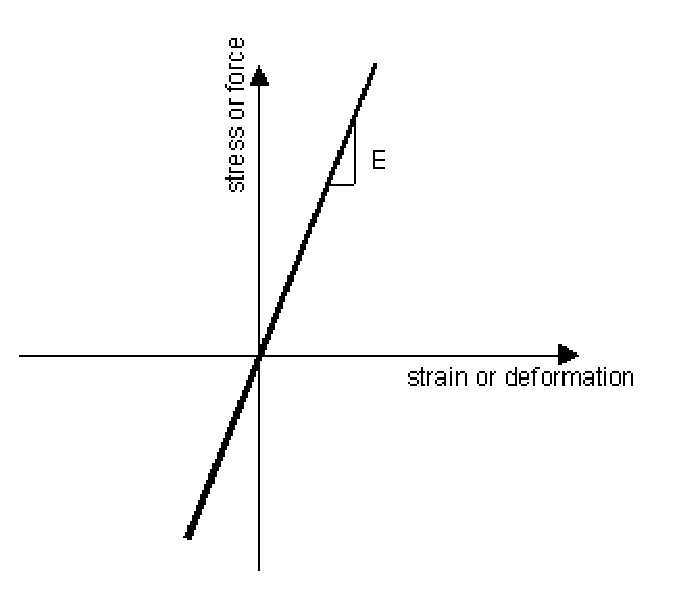
\includegraphics[width=60mm]{materials/figures/Elastic}
\caption{Elastic uniaxial material. Stress-strain diagram}\label{Elastic}
\end{figure}

\subsection{defElasticPPMaterial}
\noindent Constructs an elastic perfectly-plastic uniaxial material
\begin{verbatim}
from materials import typical_materials
typical_materials.defElasticPPMaterial(preprocessor,name,E,fyp,fyn)
\end{verbatim}
\begin{paramFuncTable}
\preprocessor{} \\
\name{material} \\
{\tt E} & tangent in the elastic zone of the stress-strain diagram (see figure \ref{ElasticPP}) \\
\fyp{} (see figure \ref{ElasticPP}) \\
\fyn{} (see figure \ref{ElasticPP}) \\
\end{paramFuncTable}

\begin{figure}[h]
\centering
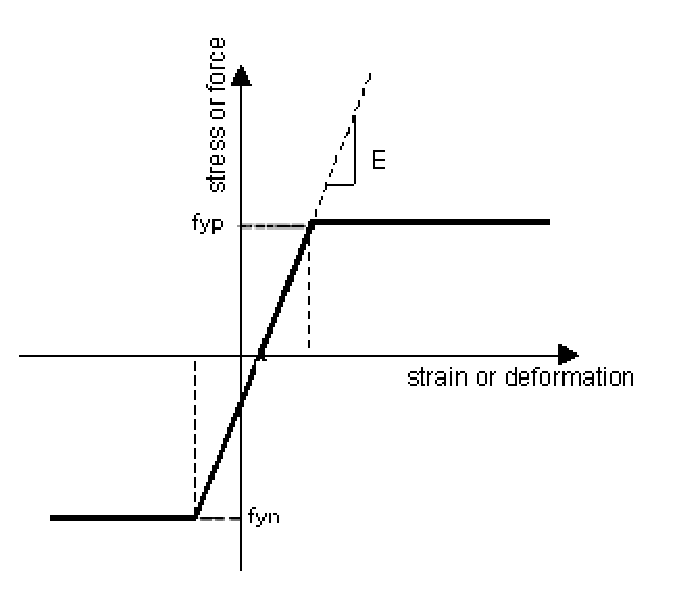
\includegraphics[width=60mm]{materials/figures/ElasticPP}
\caption{Elastic perfectly-plastic uniaxial material. Stress-strain diagram}\label{ElasticPP}
\end{figure}

\subsection{defElastNoTensMaterial}
\noindent Constructs a uniaxial elastic-no tension material
\begin{verbatim}
from materials import typical_materials
typical_materials.defElastNoTensMaterial(preprocessor,name,E)
\end{verbatim}
\begin{paramFuncTable}
\preprocessor{} \\
\name{material} \\
{\tt E} & tangent in the elastic zone of the stress-strain diagram (see figure \ref{ENT}) \\
\end{paramFuncTable}

\begin{figure}[h]
\centering
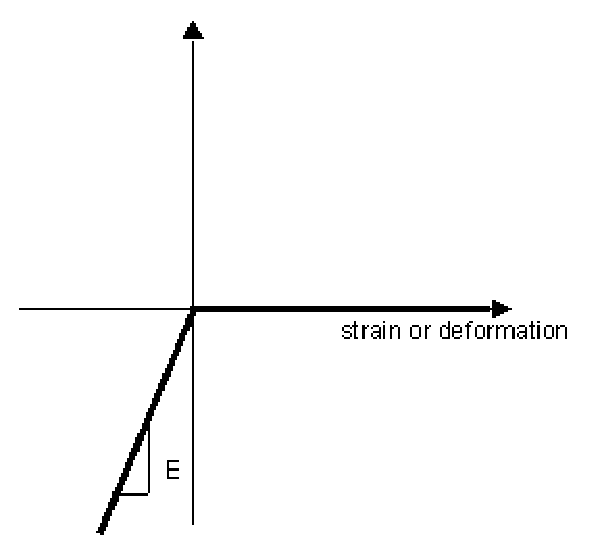
\includegraphics[width=50mm]{materials/figures/ENT}
\caption{Elastic-no tension material. Stress-strain diagram}\label{ENT}
\end{figure}

\section{Steel and reinforcing steel materials}
\subsection{defCableMaterial}
\noindent Constructs a uniaxial bilinear prestressed material. The stress strain ranges from slack (large strain at zero stress) to taught (linear with modulus E).
\begin{verbatim}
from materials import typical_materials
typical_materials.defCableMaterial(preprocessor,name,E,prestress,rho)
\end{verbatim}
\begin{paramFuncTable}
\preprocessor{} \\
\name{material} \\
\E{} \\
{\tt prestress} & prestress \\
{\tt rho} & effective self weight (gravity component of weight per volume transverse to the cable) \\
\end{paramFuncTable}


\subsection{defSteel01}
\noindent Constructs a uniaxial bilinear steel material object with kinematic hardening
\begin{verbatim}
from materials import typical_materials
typical_materials.defSteel01(preprocessor,name,E,fy,b)
\end{verbatim}
\begin{paramFuncTable}
\preprocessor{} \\
\name{material} \\
{\tt E} & initial elastic tangent (see figure \ref{Steel01}) \\
\fy{} (see figure \ref{Steel01})\\
{\tt b} &  strain-hardening ratio: ratio between post-yield tangent and initial elastic tangent (see figure \ref{Steel01})\\
\end{paramFuncTable}


\begin{figure}[h]
\centering
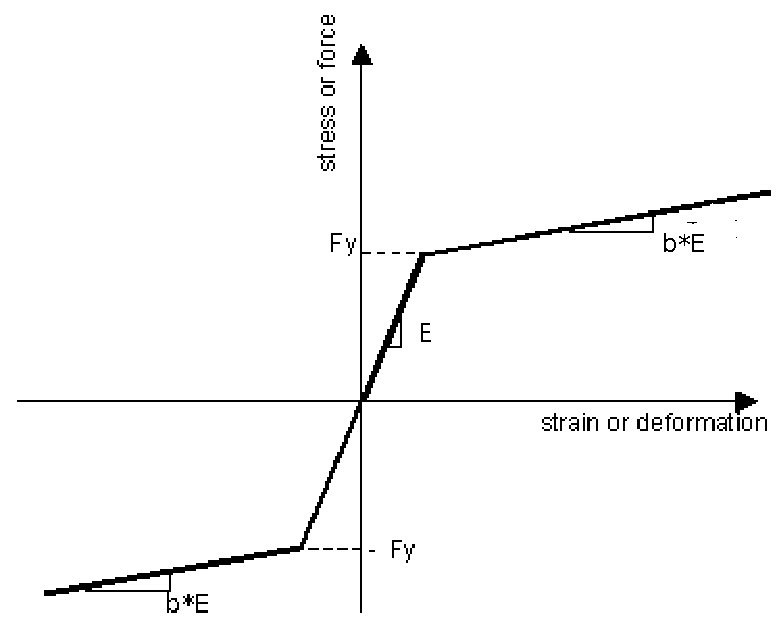
\includegraphics[width=60mm]{materials/figures/Steel01}
\caption{Steel001: uniaxial bilinear steel material with kinematic hardening. Stress-strain diagram}\label{Steel01}
\end{figure}


\subsection{defSteel02}
\noindent Constructs a uniaxial Giuffre-Menegotto-Pinto steel material object with isotropic strain hardening
\begin{verbatim}
from materials import typical_materials
typical_materials.defSteel02(preprocessor,name,E,fy,b,initialStress)
\end{verbatim}
\begin{paramFuncTable}
\preprocessor{} \\
\name{material} \\
{\tt E} & initial elastic tangent (see figure \ref{Steel02}) \\
\fy{} (see figure \ref{Steel02})\\
{\tt b} &  strain-hardening ratio: ratio between post-yield tangent and initial elastic tangent)\\
{\tt initialStress} &  initial stress \\
\end{paramFuncTable}

{\footnotesize The transition from elastic to plastic branches  (see figure \ref{Steel02}) is controlled by parameters R0, R1, R2. The default values R0=15, R1=0.925 and R2=0.15}

\begin{figure}[h]
\centering
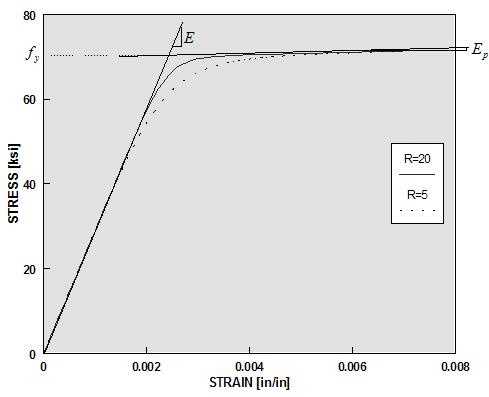
\includegraphics[width=60mm]{materials/figures/Steel02Monotonic}
\caption{Steel002: uniaxial bilinear steel material with isotropic strain hardening. Stress-strain diagram}\label{Steel02}
\end{figure}

\subsection{ReinforcingSteel}
\noindent This class constructs a bilinear stress-strain diagram to carry out the analysis of reinforced concrete according to Eurocode 2. Other national standards, like the spanish EHE and the swiss SIA also adopt this diagram.

\begin{paramClassTable}
{\tt nmbMaterial} & name identifying the material \\
{\tt nmbDiagK} & name identifying the characteristic stress-strain diagram (default: {\tt "dgK"+nmbMaterial}) \\
{\tt matTagK} & tag of the uniaxial material with the characteristic stress-strain diagram\\
{\tt nmbDiagD} &  name identifying the design stress-strain diagram (default: {\tt "dgD"+nmbMaterial}) \\
{\tt matTagD} & tag of the uniaxial material with the design stress-strain diagram\\
\fyk{} \\
{\tt gammaS} & partial factor for material (default: 1.15)\\
\Es{} of the material (default: 2e11)\\
{\tt emax} & maximum strain at failure point\\
{\tt k} & ratio between characteristic ultimate stress and characteristic yield stress $^{(1)}$ (default: 1.05)\\
\multicolumn{2}{p{13cm}}{\color{grayLines} \rule{\linewidth}{0.25pt}} \\
\multicolumn{2}{p{13cm}}{\footnotesize{(1): according to annex C of EC2: for class A k$\ge$1,05, for class B k$\ge$1,08}}
\end{paramClassTable}

\begin{methodsTable}
\fmaxk{()} \\
\fyd{()} \\
\eyk{()} \\
\eyd{()} \\
{\tt Esh()} &  post-yield tangent\\
{\tt bsh()} & ratio between post-yield tangent and initial elastic tangent\\
{\tt defDiagK(preprocessor)} & returns XC uniaxial material (characteristic values)\\
{\tt defDiagD(preprocessor)} & returns XC uniaxial material (design values)\\
\end{methodsTable}

\section{Concrete materials}
\subsection{defConcrete01}
\noindent Constructs a uniaxial Kent-Scott-Park concrete material object with degraded linear unloading/reloading stiffness according to the work of Karsan-Jirsa and no tensile strength.
\begin{verbatim}
from materials import typical_materials
typical_materials.defConcrete01(preprocessor,name,epsc0,fpc,fpcu,epscu)
\end{verbatim}
\begin{paramFuncTable}
\preprocessor{} \\
\name{material} \\
{\tt fpc} &  concrete compressive strength at 28 days (compression is negative) $^{(1)}$\\
{\tt epsc0} &  concrete strain at maximum strength (see figure \ref{Concrete01}) $^{(2)}$\\
{\tt fpcu} &  concrete crushing strength (see figure \ref{Concrete01}) \\
{\tt epscu} &  concrete strain at crushing strength (see figure \ref{Concrete01}) \\
\hline
\multicolumn{2}{p{12cm}}{\footnotesize(1): Compressive concrete parameters should be input as negative values (if input as positive, they will be converted to negative internally)}\\
\multicolumn{2}{p{12cm}}{\footnotesize (2): The initial slope for this model is $2*fpc/epsc0$ (see figure \ref{Concrete01})}\\
\end{paramFuncTable}

\begin{figure}[h]
\centering
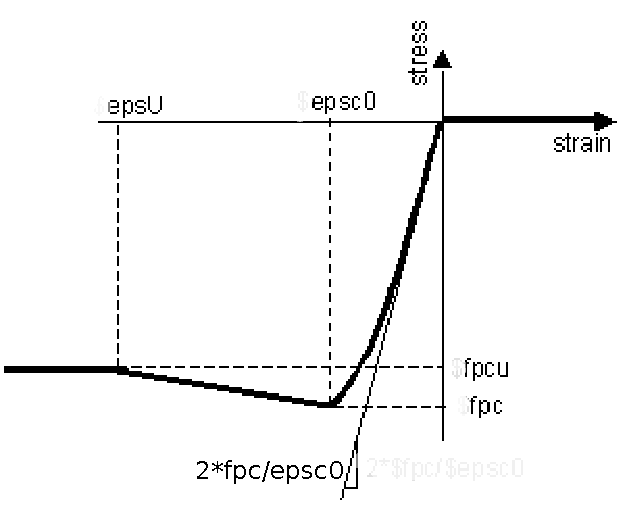
\includegraphics[width=60mm]{materials/figures/Concrete01}
\caption{Concrete01: uniaxial Kent-Scott-Park concrete material. Stress-strain diagram}\label{Concrete01}
\end{figure}

\section{ND materials}
An ND material is an object that represents the stress-strain relationship at the gauss-point of a continuum element.

\subsection{defElasticIsotropic3d}
\noindent Constructs an elastic isotropic material.
\begin{verbatim}
from materials import typical_materials
typical_materials.defElasticIsotropic3d(preprocessor,name,E,nu,rho)
\end{verbatim}
\begin{paramFuncTable}
\preprocessor{} \\
\name{material}\\
\E{} \\
\nuX{} \\
\rhoX{}, optional (default = 0.0)\\
\end{paramFuncTable}


\subsection{defElasticIsotropicPlaneStrain}
\noindent Constructs an elastic isotropic plane-strain material.
\begin{verbatim}
from materials import typical_materials
typical_materials.defElasticIsotropicPlaneStrain(preprocessor,name,E,nu,rho)
\end{verbatim}
\begin{paramFuncTable}\preprocessor{} \\
\name{material}\\
\E{} \\
\nuX \\
{\tt rho} &  mass density, optional (default = 0.0)\\
\end{paramFuncTable}


\subsection{defElasticIsotropicPlaneStress}
\noindent Constructs an elastic isotropic plane-stress material.
\begin{verbatim}
from materials import typical_materials
typical_materials.defElasticIsotropicPlaneStress(preprocessor,name,E,nu,rho)
\end{verbatim}
\begin{paramFuncTable}
\preprocessor{} \\
\name{material}\\
\E{} \\
\nuX{} \\
\rhoX{} , optional (default = 0.0)\\
\end{paramFuncTable}

\section{Sections}
A section represents a force-deformation (or resultant stress-strain) relationship at beam-column or plate element.

Three types of sections are going to be considered:
\begin{description}
\item{Elastic:} defined by material and geometric constants;
\item{Resultant:} general nonlinear description of force-deformation response, e.g. moment-curvature;
\item{Fiber:} section is discretized into smaller regions for which the material stress-strain response is integrated to give resultant behavior, e.g. reinforced concrete.
\end{description}
\subsection{Sections definition}
\subsubsection{sectionProperties}
\noindent It's an abstract class used to define the properties of a generic section.
\begin{verbatim}
from materials import sectionProperties
sectionProperties.sectionProperties(name,E,nu)
\end{verbatim}
\begin{paramClassTable}
\name{section} \\
\E{} of material\\
\nuX{} of material \\
\end{paramClassTable}
\begin{center}
\begin{tabular}{p{3.5cm}p{9cm}}
\multicolumn{2}{p{11cm}}{\color{grayText} \large{Abstract methods}} \\
\multicolumn{2}{p{13cm}}{\color{grayLines} \rule{\linewidth}{0.25pt}} \\
\A{()} (to override)\\
\Iy{()} (to override)\\
\Iz{()} (to override)\\
\J{()} (to override)\\
\G{()}  (defaults to $\cfrac{E}{2(1+\nu)}$\\
\alphaY{()} \\
\alphaZ{()} \\
\Wyel{()} \\
\Wzel{()} \\
\end{tabular}
\end{center}
\begin{methodsTable}
\multicolumn{2}{p{13cm}}{{\tt sectionProperties.defSeccElastica3d(preprocessor)}} \\
& returns an elastic section appropiate for 3D beam analysis, from the data of the section geometric properties\\
\multicolumn{2}{p{13cm}}{{\tt sectionProperties.defSeccShElastica3d(preprocessor)}} \\
& returns an elastic section appropiate for 3D beam analysis  including shear deformations, from the data of the section geometric properties\\
\multicolumn{2}{p{13cm}}{{\tt sectionProperties.defSeccElastica2d(preprocessor)}} \\
& returns an elastic section appropiate for 2D beam analysis, from the data of the section geometric properties\\
\multicolumn{2}{p{13cm}}{{\tt sectionProperties.defSeccShElastica2d(preprocessor)}} \\
& returns an elastic section appropiate for 2D beam analysis  including shear deformations, from the data of the section geometric properties\\
\end{methodsTable}

\subsubsection{defSeccElastica3d}
\noindent Returns an elastic section appropiate for 3D beam analysis.
\begin{verbatim}
from materials import sectionProperties
sectionProperties.defSeccElastica3d(preprocessor,defSecc)
\end{verbatim}
\begin{paramFuncTable}
\preprocessor{} \\
\defSecc{} \\
\end{paramFuncTable}


\subsubsection{defSeccShElastica3d}
\noindent Returns an elastic section appropiate for 3D beam analysis, including shear deformations.
\begin{verbatim}
from materials import sectionProperties
sectionProperties.defSeccShElastica3d(preprocessor,defSecc)
\end{verbatim}
\begin{paramFuncTable}
\preprocessor{} \\
\defSecc{} \\
\end{paramFuncTable}


\subsubsection{defSeccElastica2d}
\noindent Returns an elastic section appropiate for 2D beam analysis.
\begin{verbatim}
from materials import sectionProperties
sectionProperties.defSeccElastica2d(preprocessor,defSecc)
\end{verbatim}
\begin{paramFuncTable}
\preprocessor{} \\
\defSecc{} \\
\end{paramFuncTable}


\subsubsection{defSeccShElastica2d}
\noindent Returns an elastic section appropiate for 2D beam analysis, including shear deformations.
\begin{verbatim}
from materials import sectionProperties
sectionProperties.defSeccShElastica2d(preprocessor,defSecc)
\end{verbatim}
\begin{paramFuncTable}
\preprocessor{} \\
\defSecc{} \\
\end{paramFuncTable}


\subsubsection{CircularSection}
\noindent This subclass derived from superclass {\tt sectionProperties} is used to define the properties of a circular section.
\begin{verbatim}
from materials import parametrosSeccionCircular
parametrosSeccionCircular.CircularSection(name,r,E,nu)
\end{verbatim}
\begin{paramClassTable}
\name{section} \\
{\tt r} & radius \\
\E{} of material\\
\nuX of material \\
\end{paramClassTable}
\begin{methodsTable}
\A{()} \\
{\tt Iy()} &  second moment of area about the local y-axis\\
{\tt Iz()} &  second moment of area about the local z-axis\\
{\tt J()} & torsional moment of inertia of the section \\
{\tt alphaY()} & coefficient of distortion about the local y-axis\\
{\tt alphaZ()} & coefficient of distortion about the local z-axis\\
\end{methodsTable}

\begin{center}
\begin{tabular}{p{3.5cm}p{9cm}}
\multicolumn{2}{p{11cm}}{\color{grayText} \large{Functions for defining circular sections}} \\
\multicolumn{2}{p{13cm}}{\color{grayLines} \rule{\linewidth}{0.25pt}} \\
\multicolumn{2}{p{13cm}}{{\tt parametrosSeccionCircular.setupSeccCircular(sectionName,r,E,nu)}} \\
& returns a circular section \\
\multicolumn{2}{p{13cm}}{{\tt parametrosSeccionCircular.defSeccCircularElastica3d(preprocessor, defSecc)}}\\
& returns an elastic circular section appropiate for 3D beam analysis.\\
\multicolumn{2}{p{13cm}}{{\tt parametrosSeccionCircular.defSeccCircularShElastica3d(preprocessor, defSecc)}}\\
& returns an elastic circular section appropiate for 3D beam analysis, including shear deformations.\\
\multicolumn{2}{p{13cm}}{{\tt parametrosSeccionCircular.defSeccCircularElastica2d(preprocessor, defSecc)}}\\
& returns an elastic circular section appropiate for 2D beam analysis.\\
\multicolumn{2}{p{13cm}}{{\tt parametrosSeccionCircular.defSeccCircularShElastica2d(preprocessor, defSecc)}}\\
& returns an elastic circular section appropiate for 2D beam analysis, including shear deformations.\\
& {\tt preprocessor} : preprocessor name \\
& {\tt defSecc} : name identifying an object of the class {\tt CircularSection} with the properties of the section. \\
\end{tabular}
\end{center}

\subsubsection{RectangularSection}
\noindent This subclass derived from superclass {\tt sectionProperties} is used to define the properties of a rectangular section.
\begin{verbatim}
from materials import parametrosSeccionRectangular
parametrosSeccionRectangular.RectangularSection(,name,b,h,E,nu)
\end{verbatim}
\begin{paramClassTable}
\name{section} \\
\bX{} \\
\h{} \\
\E{} of material\\
\nuX of material \\
\end{paramClassTable}
\begin{methodsTable}
\A(){} \\
\Iy{()}  (Y= weak axis)\\
\Iz{()}  (Z= strong axis)\\
\J{()} \\
\Wyel{()}\\
\Wzel{()} \\
\alphaY{()}\\
\alphaZ{()}\\
\end{methodsTable}

\begin{center}
\begin{tabular}{p{3.5cm}p{9cm}}
\multicolumn{2}{p{11cm}}{\color{grayText} \large{Functions for defining parameters of rectangular sections}} \\
\multicolumn{2}{p{13cm}}{\color{grayLines} \rule{\linewidth}{0.25pt}} \\
\multicolumn{2}{p{13cm}}{{\tt parametrosSeccionRectangular.getJTorsion( b, h)}} \\
& returns the torsional moment of inertia of the rectangular section \\
\end{tabular}
\end{center}

\subsubsection{sccRectang}
\noindent This class is used to define a geometric rectangular section.
\begin{verbatim}
from materials import sccRectg
sccRectg.sccRectang()
\end{verbatim}
\begin{paramClassTable}
\bX{} \\
\h{} \\
\nDivIJ{} \\
\nDivJK{} \\
\end{paramClassTable}
\begin{methodsTable}
{\tt area()} & rectangle area \\
\IAxisOne{()} \\
\iAxisOne{()} \\
\MeAxisOne{(fy)} {\tt fy} = yield stress of the section material \\
{\tt  S1PosG()} & first moment of the area of half a section with regard to the axis 1 \\
{\tt Mp1(fy)} & plastic moment of the rectangular section about the axis 1 {\tt fy} = yield stress of the section material \\
\IAxisTwo{()} \\
\iAxisTwo{()} \\
{\tt Me2(fy)} & yield moment of the rectangular section about the axis 2 {\tt fy} = yield stress of the section material \\
{\tt  S2PosG()} & first moment of the area of half a section with regard to the axis 2 \\
{\tt Mp2(fy)} & plastic moment of the rectangular section about the axis 2 {\tt fy} = yield stress of the section material \\
\multicolumn{2}{l}{\tt discretization(gm,nmbMat)} \\
& returns the discretized region \\
& {\tt gm}: name identifying a section geometry \\
& {\tt nmbMat}: name identifying the material \\ 
\end{methodsTable}

\subsubsection{SteelProfile}
\noindent This subclass derived from superclass {\tt sectionProperties} is used to define the properties of a structural steel section.
\begin{verbatim}
from materials import steelProfile
steelProfile.SteelProfile(steel,name,table)
\end{verbatim}
\begin{paramClassTable}
{\tt steel} & type of structural steel (e.g. {\tt S275JR}) \\
{\tt table} & file containing a table (dictionary) of steel profiles (e.g. {\tt perfiles\_metalicos.arcelor.perfiles\_he\_arcelor})\\
{\tt name} & name of the profile in the table (e.g. {\tt "HE\_400\_B"}) \\
\end{paramClassTable}
\begin{methodsTable}
\A{()} \\
\Iy{()} (Y= weak axis)\\
\Iz{()}  (Z= strong axis)\\
\J{()} \\
\EIy{()}\\
\EIz{()}\\
\GJ{()}\\
\alphaY{()}\\
\alphaZ{()}\\
\end{methodsTable}

\subsection{Elastic sections}
\subsubsection{defElasticSection2d}
\noindent Constructs an elastic section appropiate for 2D beam analysis.
\begin{verbatim}
from materials import typical_materials
typical_materials.defElasticSection2d(preprocessor,name,A,E,I)
\end{verbatim}
\begin{paramFuncTable}
\preprocessor{} \\
\name{section} \\
\A{} \\
{\tt E} &  Young's modulus of material \\
{\tt I} &  second moment of area about the local z-axis\\
\end{paramFuncTable}



\subsubsection{defElasticShearSection2d}
\noindent Constructs an elastic section appropiate for 2D beam analysis, including shear deformations.
\begin{verbatim}
from materials import typical_materials
typical_materials.defElasticShearSection2d(preprocessor,name,A,E,G,I,alpha)
\end{verbatim}
\begin{paramFuncTable}
\preprocessor{} \\
\name{section} \\
\A{} \\
{\tt E} &  Young's modulus of material \\
{\tt G} & shear modulus \\
{\tt I} &  second moment of area about the local z-axis\\
{\tt alpha} & shear shape factor \\
\end{paramFuncTable}


\subsubsection{defElasticSectionFromMechProp2d}
\noindent Constructs an elastic section appropiate for 2D beam analysis, taking mechanical properties of the section form a MechProp2d object.
\begin{verbatim}
from materials import typical_materials
typical_materials.defElasticSectionFromMechProp2d(preprocessor,name,mechProp2d)
\end{verbatim}
\begin{paramFuncTable}
\preprocessor{} \\
\name{section} \\
{\tt mechProp2d} & object that contains mechanical properties of the section  \\
\end{paramFuncTable}

%%%
\subsubsection{defElasticSection3d}
\noindent Constructs an elastic section appropiate for 3D beam analysis.
\begin{verbatim}
from materials import typical_materials
typical_materials.defElasticSection3d(preprocessor,name,A,E,G,Iz,Iy,J)
\end{verbatim}
\begin{paramFuncTable}
\preprocessor{} \\
\name{section} \\
\A{} \\
\E{} of material \\
\Iz{} \\
\Iy{} \\
\J{}\\
\end{paramFuncTable}


\subsubsection{defElasticShearSection3d}
\noindent Constructs an elastic section appropiate for 3D beam analysis, including shear deformations.
\begin{verbatim}
from materials import typical_materials
typical_materials.defElasticShearSection3d(preprocessor,name,A,E,G,Iz,Iy,J,alpha)
\end{verbatim}
\begin{paramFuncTable}
\preprocessor{} \\
\name{section} \\
\A{} \\
\E of material \\
\G{} \\
\Iz{} \\
\Iy{} \\
\J{} \\
\alphaX{} \\
\end{paramFuncTable}

\subsubsection{defElasticSectionFromMechProp3d}
\noindent Constructs an elastic section appropiate for 3D beam analysis, taking mechanical properties of the section form a MechProp3d object.
\begin{verbatim}
from materials import typical_materials
typical_materials.defElasticSectionFromMechProp3d(preprocessor,name,mechProp3d)
\end{verbatim}
\begin{paramFuncTable}
\preprocessor{} \\
\name{section} \\
{\tt mechProp3d} & object that contains mechanical properties of the section  \\
\end{paramFuncTable}


\subsubsection{defElasticMembranePlateSection}
\noindent Constructs an an isotropic elastic section appropriate for plate and shell analysis.
\begin{verbatim}
from materials import typical_materials
typical_materials.defElasticMembranePlateSection(preprocessor,name,E,nu,rho,h)
\end{verbatim}
\begin{paramFuncTable}
\preprocessor{} \\
\name{section}\\
\E{} \\
\nuX{} \\
\rhoX{} \\
\h{} of section\\
\end{paramFuncTable}

\subsubsection{defElasticPlateSection}
\noindent Constructs an an isotropic elastic section appropriate for plate analysis.
\begin{verbatim}
from materials import typical_materials
typical_materials.defElasticPlateSection(preprocessor,name,E,nu,rho,h)
\end{verbatim}
\begin{paramFuncTable}
\preprocessor{} \\
\name{section}\\
\E{} \\
\nuX{}\\
\rhoX{} \\
\h{} of section\\
\end{paramFuncTable}

\subsection{Fiber sections}
\subsubsection{FiberSet}
\noindent This class constructs a set of all the  fibers made of the same material from a fiber section
\begin{verbatim}
from materials.fiber_section import createFiberSets
createFiberSets.FiberSet(scc,setName,matTag)
\end{verbatim}
\begin{paramClassTable}
{\tt scc} & name identifying the fiber section \\
{\tt setName} & name of the set of fibers to be generated \\
{\tt matTag} & tag of the uniaxial material which forms the fibers \\
\end{paramClassTable}

\begin{methodsTable}
\multicolumn{2}{p{13cm}}{{\tt getFiberWithMinStrain()}}  \\
 & returns the fiber with the minimum straim from the set of fibers \\
\multicolumn{2}{p{13cm}}{{\tt getFiberWithMaxStrain()}}  \\
 & returns the fiber with the maximum straim from the set of fibers \\
\end{methodsTable}


\subsubsection{RCSets}
\noindent This class constructs both the concrete and reinforced steel fiber sets from a reinforced concrete fiber section.
\begin{verbatim}
from materials.fiber_section import createFiberSets
createFiberSets.RCSets(scc,concrMatTag, concrSetName,reinfMatTag, reinfSetName)
\end{verbatim}
\begin{paramClassTable}
{\tt scc} & name identifying the fiber section \\
{\tt concrMatTag} & tag of the uniaxial material that makes up the concrete fibers of the section \\
{\tt concrSetName} & name of the set of fibers of concrete to be generated \\
{\tt reinfMatTag} & tag of the uniaxial material that makes up the reinforcing steel fibers of the section \\
{\tt reinfSetName} & name of the set of fibers of reinforcing steel to be generated \\
\end{paramClassTable}

\begin{methodsTable}
\multicolumn{2}{p{13cm}}{{\tt reselTensionFibers(scc,tensionFibersSetName)}} \\
& returns a set with those fibers in tension from the total set \\
\multicolumn{2}{p{13cm}}{{\tt getConcreteArea(factor)}} \\
 & returns the cross section area of concrete in the set \\
\multicolumn{2}{p{13cm}}{{\tt getMaxConcreteStrain()}} \\
 & returns the maximum strain in the set of concrete fibers \\
\multicolumn{2}{p{13cm}}{{\tt getConcreteInitialTangent()}} \\
 & returns the initial tangent in the stress-strain diagram of the material that makes up the fibers of concrete \\
\multicolumn{2}{p{13cm}}{{\tt getConcreteCompression()}} \\
 & returns the resultant of compressive stresses in concrete fibers \\
\multicolumn{2}{p{13cm}}{{\tt getNumTensionRebars()}} \\
 & returns the number of reinforcing steel fibers in tension \\
\end{methodsTable}

\subsubsection{fiberSectionSetupRCSets}
Returns an object of the class \verb|RCSets|
\begin{verbatim}
from materials.fiber_section import createFiberSets
createFiberSets.fiberSectionSetupRCSets(scc,concrMatTag, concrSetName,reinfMatTag, reinfSetName)
\end{verbatim}
\begin{paramFuncTable}
{\tt scc} & name identifying the fiber section \\
{\tt concrMatTag} & tag of the uniaxial material that makes up the concrete fibers of the section \\
{\tt concrSetName} & name of the set of fibers of concrete to be generated \\
{\tt reinfMatTag} & tag of the uniaxial material that makes up the reinforcing steel fibers of the section \\
{\tt reinfSetName} & name of the set of fibers of reinforcing steel to be generated \\
\end{paramFuncTable}


\subsubsection{createRCFiberSets}
Constructs the sets of concrete fibers (\verb|"hormigon"|) and reinforcing steel fibers (\verb|"armadura"|) for all the elements included in a set of elements.
\begin{verbatim}
from materials.fiber_section import createFiberSets
createFiberSets.createRCFiberSets(preprocessor, setName, concrMatTag, reinfMatTag)
\end{verbatim}
\begin{paramFuncTable}
\preprocessor{} \\
{\tt setName} & name identifying the set of elements \\
{\tt concrMatTag} & tag of the uniaxial material that makes up the concrete fibers of the section \\
{\tt reinfMatTag} & tag of the uniaxial material that makes up the reinforcing steel fibers of the section \\
\end{paramFuncTable}

\subsubsection{reselTensionFibers}
Returns the fibers under tension included in a set of fibers.
\begin{verbatim}
from materials.fiber_section import createFiberSets
createFiberSets.reselTensionFibers(scc,fiberSetName,tensionFibersSetName)
\end{verbatim}
\begin{paramFuncTable}
{\tt scc} & name identifying the fiber section \\
{\tt fiberSetName} & name identifying the set of fibers \\
{\tt tensionFibersSetName} & name of the set of tensioned fibers returned\\
\end{paramFuncTable}


\subsubsection{fiberSectionSetupRC3Sets}
Returns a set of tensioned fibers (\verb|"armaduraTraccion"|) of a fiber section of reinforced concrete.
\begin{verbatim}
from materials.fiber_section import createFiberSets
createFiberSets.fiberSectionSetupRC3Sets(scc,concrMatTag, concrSetName,reinfMatTag, reinfSetName)
\end{verbatim}
\begin{paramFuncTable}
{\tt scc} & name identifying the fiber section \\
{\tt concrMatTag} & tag of the uniaxial material that makes up the concrete fibers of the section \\
{\tt concrSetName} & name of the set of fibers of concrete to be generated \\
{\tt reinfMatTag} & tag of the uniaxial material that makes up the reinforcing steel fibers of the section \\
{\tt reinfSetName} & name of the set of fibers of reinforcing steel to be generated \\
\end{paramFuncTable}


\subsubsection{RecordRCColumnSection}
\noindent This class is used to define the variables that make up a reinforced concrete section with reinforcement symmetric in both directions (as usual in columns)
\begin{verbatim}
from materials.fiber_section import defSeccionHAPilar
defSeccionHAPilar.RecordRCColumnSection()
\end{verbatim}
\begin{paramClassTable}
{\tt sectionName} & name identifying the section \\
{\tt sectionDescr} & section description \\
{\tt gmSectionName} & name identifying the geometric section \\
{\tt concrType} & type of concrete (e.g. hormigonesEHE.HA25) \\
{\tt concrDiagName} & name identifying the characteristic stress-strain diagram of the concrete material \\
{\tt depth} & cross-section depth \\
{\tt width} & cross-section width \\
\nDivIJ{}\\
\nDivJK{} \\
{\tt reinfSteelType} & type of reinforcement steel \\
{\tt reinfDiagName} & name identifying the characteristic stress-strain diagram of the reinforcing steel material \\
{\tt cover} & cover \\
{\tt nRebarsWidth} & number of rebars in the width direction of the section (each face)\\
{\tt areaRebarWidth} & cross sectional area of each rebar in  width direction \\
{\tt nRebarsDepth} & number of rebars in the height direction of the section (each face )\\
{\tt areaRebarDepth} & cross sectional area of each rebar in height direction \\
{\tt shReinfZ} & record of type {\tt defSeccionHASimple.RecordShearReinforcement()} defining the shear reinforcement in Z direction \\
{\tt shReinfY} & record of type {\tt defSeccionHASimple.RecordShearReinforcement()} defining the shear reinforcement in Y direction \\
\end{paramClassTable}

\begin{methodsTable}
\multicolumn{2}{p{13cm}}{{\tt defGeomRCColumnSection(matDiagType)}} \\
 & returns a reinforced concrete section with reinforcement symmetric in both directions \\
& {\tt matDiagType} ="k" for characteristic diagram, ="d" for design diagram \\ 
\end{methodsTable}

\subsubsection{RecordShearReinforcement}
\noindent This class is used to define the variables that make up a family of shear reinforcing bars.
\begin{verbatim}
from materials.fiber_section import defSeccionHASimple
defSeccionHASimple.RecordShearReinforcement()
\end{verbatim}
\begin{paramClassTable}
{\tt familyName} & name identifying the family of shear reinforcing bars \\
{\tt nShReinfBranches} & number of effective branches\\
{\tt areaShReinfBranch} &  area of the shear reinforcing bar\\
{\tt shReinfSpacing} & longitudinal distance between transverse reinforcements (defaults to 0.2)\\
{\tt angAlphaShReinf} & angle between the shear reinforcing bars and the axis of the member (defaults to $\Pi/2$)\\
{\tt angThetaConcrStruts} & angle between the concrete's compression struts and the axis of the member (defaults to $\Pi/4$)\\
\end{paramClassTable}
\begin{methodsTable}
{\tt getAs()} & returns the area per unit length of the family of shear reinforcements\\
\end{methodsTable}

\subsubsection{RecordRCSimpleSection}
\noindent This class is used to define the variables that make up a rectangular reinforced concrete section with single reinforcement layers in top and bottom faces
\begin{verbatim}
from materials.fiber_section import defSeccionHASimple
defSeccionHASimple.RecordRCSimpleSection()
\end{verbatim}
\begin{paramClassTable}
{\tt sectionName} & name identifying the section \\
{\tt sectionDescr} & section description \\
{\tt tipoHormigón} & type of concrete (e.g. hormigonesEHE.HA25) \\
{\tt concrDiagName} & name identifying the characteristic stress-strain diagram of the concrete material \\
{\tt depth} & cross-section height \\
{\tt width} & cross-section width \\
\nDivIJ{} \\
\nDivJK{} \\
{\tt reinfSteelType} & type of reinforcement steel \\
{\tt reinfDiagName} & name identifying the characteristic stress-strain diagram of the reinforcing steel material \\
{\tt nRebarsNeg} & number of longitudinal rebars in the negative face of the section\\
{\tt areaRebarNeg} & area of each longitudinal rebar in  the negative face \\
{\tt rebarsDiamNeg} & diameter of the bars in  the negative face of the section \\
{\tt coverNeg} & cover of longitudinal reinforcement in the negative face\\
{\tt coverLatNeg} & lateral cover of longitudinal reinforcement in the negative face\\
{\tt nRebarsPos} & number of longitudinal rebars in the positive face of the section\\
{\tt areaRebarPos} & area of each longitudinal rebar in  the positive face \\
{\tt rebarsDiamPos} & diameter of the bars rebar in  the positive face of the section \\
{\tt coverPos} & cover of longitudinal reinforcement in the positive face\\
{\tt coverLatPos} & lateral cover of longitudinal reinforcement in the positive face\\
{\tt coverMin} & minimal covering of the longitudinal reinforcement \\
{\tt shReinfZ} & record of type {\tt defSeccionHASimple.RecordShearReinforcement()} defining the shear reinforcement in Z direction \\
{\tt shReinfY} & record of type {\tt defSeccionHASimple.RecordShearReinforcement()} defining the shear reinforcement in Y direction \\
\end{paramClassTable}
\begin{methodsTable}
\multicolumn{2}{p{13cm}}{{\tt defGeomRCColumnSection(matDiagType)}} \\
 & returns a reinforced concrete section with reinforcement symmetric in both directions \\
& {\tt matDiagType} ="k" for characteristic diagram, ="d" for design diagram \\ 
\end{methodsTable}


\subsubsection{RecordRCSlabSection}
\noindent This class is used to define the variables that make up a reinforced concrete slab section with single reinforcement layers in top and bottom faces
\begin{verbatim}
from materials.fiber_section import defSeccionHASimple
defSeccionHASimple.RecordRCSlabSection(nmb,desc,depth,concrete,steel,basicCover)
\end{verbatim}
\begin{paramClassTable}
{\tt nmb} & basic name identifying the section \\
& the name identifying the section in 1 direction is formed adding to {\tt nmb} the suffix  "L"; for the section in 2 direction the suffix added to the basic name is "T" \\
{\tt desc} & basic section description \\
{\tt depth} & cross-section height (width is considered = 1)\\
{\tt concrete} & type of concrete (e.g. hormigonesEHE.HA25) \\
{\tt steel} & type of reinforcement steel \\
{\tt basicCover} & minimal cover of longitudinal reinforcement \\
\end{paramClassTable}

\begin{methodsTable}
\multicolumn{2}{p{13cm}}{{\tt setMainReinf2neg(diam,area,spacing)}} \\
 & defines the rebar arrangement of the layer of main reinforcement bars corresponding to the negative face of the section in 2 direction \\
& {\tt diam} = diameter of the bar \\
& {\tt area} = area of each bar \\
& {\tt spacing} = space between axis of bars \\
\multicolumn{2}{p{13cm}}{{\tt setMainReinf2pos(diam,area,spacing)}} \\
 & \emph{idem} for the layer of main reinforcement bars corresponding to the positive face of the section in 2 direction \\
\multicolumn{2}{p{13cm}}{{\tt setMainReinf1neg(diam,area,spacing)}} \\
 & \emph{idem} for the layer of main reinforcement bars corresponding to the negative face of the section in 1 direction \\
\multicolumn{2}{p{13cm}}{{\tt setMainReinf1pos(diam,area,spacing)}} \\
 & \emph{idem} for the layer of main reinforcement bars corresponding to the positive face of the section in 1 direction \\
\multicolumn{2}{p{13cm}}{{\tt setShearReinfT(nShReinfBranches,areaShReinfBranch,spacing)}} \\
 & defines the rebar arrangement of the shear reinforcement bars corresponding to the section in 2 direction \\
& {\tt nShReinfBranches} =  number of effective branches \\
& {\tt areaShReinfBranch} = area of the shear reinforcing bar \\
& {\tt spacing} = longitudinal distance between shear reinforcements bars \\
\multicolumn{2}{p{13cm}}{{\tt setShearReinfL(nShReinfBranches,areaShReinfBranch,spacing)}} \\
 & \emph{idem} for shear reinforcement bars corresponding to the section in 1 direction \\
\end{methodsTable}

\subsubsection{getIMaxPropFiber}
Returns the fiber in a set with the maximum value of a property.
\noindent 
\begin{verbatim}
from materials.fiber_section import fiberUtils
fiberUtils.getIMaxPropFiber(fibers,methodName)
\end{verbatim}
\begin{paramFuncTable}
{\tt fibers} & name of the set of fibers \\
{\tt methodName} & name of the method or property (e.g. {\tt "getArea"}) \\
\end{paramFuncTable}


\subsubsection{getIMinPropFiber}
Returns the fiber with the minimum value of a property from a set of fibers.
\noindent 
\begin{verbatim}
from materials.fiber_section import fiberUtils
fiberUtils.getIMinPropFiber(fibers,methodName)
\end{verbatim}
\begin{paramFuncTable}
{\tt fibers} & name of the set of fibers \\
{\tt methodName} & name of the method or property (e.g. {\tt "getArea"}) \\
\end{paramFuncTable}



\subsubsection{Utils}
\paragraph{tipoSolicitacion}
\noindent Returns the following values, depending on the state of stress in the section:
\begin{description}
\item{1} pure or combined tension where the entire section is under tension;
\item{2} pure or combined bending (there are fibers in tension and in compression);
\item{3} single or combined compression where all the fibers are in compression.
\end{description}
\begin{verbatim}
from materials import regimenSeccion
regimenSeccion.tipoSolicitacion(epsCMin, epsSMax)
\end{verbatim}
\begin{paramFuncTable}
\epsCMin{}\\
\epsSMax{}\\
\end{paramFuncTable}


\paragraph{strTipoSolicitacion}
\noindent Returns:
\begin{description}
\item{\verb|"tracción simple o compuesta"|} in pure or combined tension state;
\item{\verb|"flexotracción"|} in pure or combined bending state;
\item{\verb|"compresión simple o compuesta"|} in single or combined compression state;
\item{\verb|"falla"|} in all other cases.
\end{description}
\begin{verbatim}
from materials import regimenSeccion
regimenSeccion.strTipoSolicitacion(tipoSol)
\end{verbatim}
\begin{paramFuncTable}
{\tt tipoSol} & =1 for pure or combined tension state \\
& =2 for pure or combined bending state \\
& =3 for single or combined compression state \\
\end{paramFuncTable}

\subsubsection{gmHorizRowRebars}
Returns a reinforcement layer parallel to the top and bottom sides of the rectangular section. The row of reinforcement bars is placed at a distance {\tt h} over the horizontal axis of the section. 
\noindent 
\begin{verbatim}
from materials.fiber_section import geomArmaduraSeccionesFibras
geomArmaduraSeccionesFibras.gmHorizRowRebars(sectionGeom, fiberMatName, 
nRebars, areaRebar, depth, width, cover, h)
\end{verbatim}
\begin{paramFuncTable}
{\tt sectionGeom} & name identifying the geometric section \\
{\tt fiberMatName} & name identifying the uniaxial material which forms the fibers\\
{\tt nRebars} & number of rebars in the layer \\
{\tt areaRebar} &  area of each rebar \\
{\tt depth} &  cross-section height \\
{\tt width} & cross-section width \\
{\tt cover} & cover \\
{\tt h} & distance between the horizontal axis of the cross-section and the reinforcement layer \\
\end{paramFuncTable}

\subsubsection{gmBottomRowRebars}
Returns a reinforcement layer in the bottom side of a rectangular section.
\noindent 
\begin{verbatim}
from materials.fiber_section import geomArmaduraSeccionesFibras
geomArmaduraSeccionesFibras.gmBottomRowRebars(sectionGeom,fiberMatName, 
nRebars, areaRebar, depth, width, cover)
\end{verbatim}
\begin{paramFuncTable}
{\tt sectionGeom} & name identifying the geometric section \\
{\tt fiberMatName} & name identifying the uniaxial material which forms the fibers\\
{\tt nRebars} & number of rebars in the layer \\
{\tt areaRebar} &  area of each rebar \\
{\tt depth} &  cross-section height \\
{\tt width} & cross-section width \\
{\tt cover} & cover \\
\end{paramFuncTable}

\subsubsection{ggmTopRowRebars}
Returns a reinforcement layer in the top side of a rectangular section.
\noindent 
\begin{verbatim}
from materials.fiber_section import geomArmaduraSeccionesFibras
geomArmaduraSeccionesFibras.ggmTopRowRebars(sectionGeom,fiberMatName, 
nRebars, areaRebar, depth, width, cover)
\end{verbatim}
\begin{paramFuncTable}
{\tt sectionGeom} & name identifying the geometric section \\
{\tt fiberMatName} & name identifying the uniaxial material which forms the fibers\\
{\tt nRebars} & number of rebars in the layer \\
{\tt areaRebar} &  area of each rebar \\
{\tt depth} &  cross-section height \\
{\tt width} & cross-section width \\
{\tt cover} & cover \\
\end{paramFuncTable}

\subsubsection{gmSquareSection}
Returns a square geometric region of fibers' material.
\noindent 
\begin{verbatim}
from materials.fiber_section import geomSeccionesFibras
geomSeccionesFibras.gmSquareSection(geomSection, fiberMatName, ld, nD)
\end{verbatim}
\begin{paramFuncTable}
{\tt geomSection} & name identifying the geometric section \\
{\tt fiberMatName} & name identifying the uniaxial material which forms the fibers\\
{\tt ld} & side of the square \\
{\tt nD} & number of cells in each side of the square \\
\end{paramFuncTable}

\subsubsection{gmRectangSection}
Returns a rectangular geometric region of fibers' material.
\noindent 
\begin{verbatim}
from materials.fiber_section import geomSeccionesFibras
geomSeccionesFibras.gmRectangSection(geomSection,fiberMatName, h, b, 
nDIJ, nDIK)
\end{verbatim}
\begin{paramFuncTable}
{\tt geomSection} & name identifying the geometric section \\
{\tt fiberMatName} & name identifying the uniaxial material which forms the fibers\\
{\tt h} & side of the rectangle in IK direction \\
{\tt b} & side of the rectangle in IJ direction \\
{\tt nDIJ} & number of cells in IJ direction \\
{\tt nDIK} & number of cells in IK direction \\
\end{paramFuncTable}


\subsubsection{RecordFamArmaduraPrincipal}
\noindent This class constructs a family of main reinforcing bars.
\begin{verbatim} materials.fiber_section import informeGeomSeccion
informeGeomSeccion.RecordFamArmaduraPrincipal(reinfLayer)
\end{verbatim}

\begin{paramClassTable}
{\tt reinfLayer} & name identifying the family of reinforcing bars \\
{\tt nRebars} & number of rebars in the layer \\
{\tt rebarsDiam} & diameter of the bars \\
{\tt areaRebar} & total area of the bars in the family \\
{\tt coverMec} & cover of the reinforcement\\
{\tt cdgBarras} & position of the reinforcement centre of gravity \\
\end{paramClassTable}

\begin{methodsTable}
\multicolumn{2}{p{13cm}}{{\tt texWrite(archTex)}} \\
& writes the value of parameters in a file named {\tt archTex} \\ 
\end{methodsTable}

\subsubsection{imprimeArmaduraPrincipal}
\noindent The function writes in the specified file the characteristics (diameter, area, cover, position of gravity centre, \ldots) of each main reinforcement family provided in a list of family names.
\begin{verbatim}
from materials.fiber_section import informeGeomSeccion
informeGeomSeccion.imprimeArmaduraPrincipal(listaFamArmaduraPrincipal, 
areaHorm, archTex)
\end{verbatim}
\begin{paramFuncTable}
{\tt listaFamArmaduraPrincipal} & name identifying a list of names of reinforcement families \\
{\tt areaHorm} & area of the concrete section \\
{\tt archTex} &  name of the output file \\
\end{paramFuncTable}

\subsubsection{imprimeArmaduraCortante}
\noindent The function writes in the specified file the characteristics (diameter, area, distances, angles, \ldots) of a family of shear reinforcement bars.
\begin{verbatim}
from materials.fiber_section import informeGeomSeccion
informeGeomSeccion.imprimeArmaduraCortante(recordArmaduraCortante, 
archTex)
\end{verbatim}
\begin{paramFuncTable}
{\tt recordArmaduraCortante} & name identifying a family of shear reinforcement \\
{\tt archTex} &  name of the output file \\
\end{paramFuncTable}


\subsubsection{informeGeomSeccion}
\noindent This function prepares a report with the characteristics of a sections, as illustrated in table \ref{informSec}
\begin{verbatim}
from materials.fiber_section import informeGeomSeccion
informeGeomSeccion.informeGeomSeccion(preprocessor,scc, archTex, pathFigura)
\end{verbatim}
\begin{paramFuncTable}
\preprocessor{} \\
{\tt scc} & name identifying the section \\
{\tt archTex} &  name of the output file \\
{\tt pathFigura} & path to place the figure file representing the reinforcement arrangement \\
\end{paramFuncTable}

\begin{table}
\begin{center}
\begin{tabular}{|c|}
\hline
\begin{large} PI\_PF\_OD\_100\_39SecHA1HstICent \end{large}\\
\hline
Sección central en hastial izquierdo. Armadura vertical.\\
\hline
\begin{tabular}{c|l}
\begin{minipage}{85mm}
\vspace{2mm}
\begin{center}
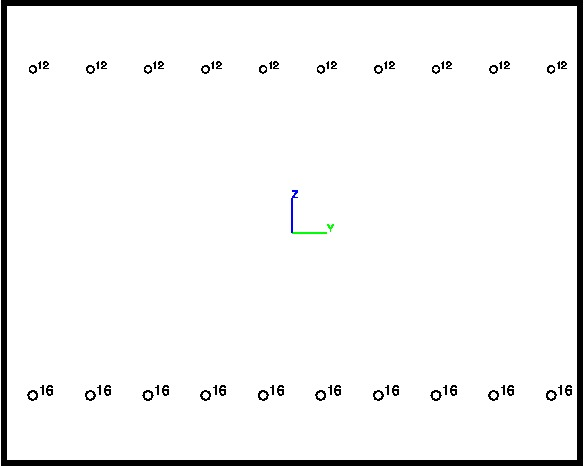
\includegraphics[width=80mm]{materials/figures/hsticentDatosScc1}
\end{center}
\vspace{1pt}
\end{minipage} & 
\begin{tabular}{l}
width: \\
$b= 1.00\ m$\\
depth: \\
$h= 0.70\ m$\\
\end{tabular} \\
\end{tabular} \\
\hline
\textbf{Materiales}:\\
\hline
\begin{tabular}{ll}
Hormigón: HA30 & Módulo de deformación longitudinal: $E_c= 28.58\ GPa$\\
\hline
Acero: B500S & Módulo elástico: $E_s= 200.00\ GPa$\\
\end{tabular} \\
\hline
\textbf{Valores estáticos}:\\
\hline
Sección bruta:\\
\hline
\begin{tabular}{ll}
$A_{bruta}= 0.700\ m^2$ & \multirow{3}{*}{Tensor de inercia ($cm^4$): $ \left( \begin{array}{ccc}647.78 & 0.00 & 0.00 \\ 0.00 & 285.83 & -0.00 \\ 0.00 & -0.00 & 583.33 \end{array} \right)$} \\
& \\
C.D.G.: $( 0.00, 0.00)\ m$  & \\
\end{tabular} \\
\hline
Sección homogeneizada:\\
\hline
\begin{tabular}{ll}
$A_{homog.}= 0.737\ m^2$ & \multirow{3}{*}{Tensor de inercia ($cm^4$): $ \left( \begin{array}{ccc}647.78 & 0.00 & 0.00 \\ 0.00 & 315.25 & -0.00 \\ 0.00 & -0.00 & 613.81 \end{array} \right)$} \\
& \\
C.D.G.: $( 0.00,-0.00)\ m$  & \\
\end{tabular} \\
\hline
\textbf{Armadura pasiva}:\\
\hline
\begin{tabular}{ll}
Área total $A_s=31.40\ cm^2$ & Cuantía geométrica $\rho= 4.49\permil$\\
\end{tabular} \\
\hline
Familias de reinforcement principal:\\
\hline
\begin{tabular}{cccccccc}
Id & n. barras & $\phi$ & área & c. geom. & cover. mec. & $y_{cdg}$ & $z_{cdg}$\\
 &  & $(mm)$ & $(cm^2)$ & $(\permil)$ & $(cm)$ & $(m)$ & $(m)$\\
\hline
neg & 10 & 16 & 20.10 & 2.87 &  5.0 & 0.000 & -0.282\\
\hline
pos & 10 & 12 & 11.30 & 1.61 &  5.0 & 0.000 & 0.284\\
\end{tabular} \\
\hline
Familias de reinforcement de cortante:\\
\hline
\begin{tabular}{cccccccc}
Id & n. ramas & $\phi$ & área & sep. & area/m & $\alpha$ & $\beta$\\
 &  & $(mm)$ & $(cm^2)$ & $(cm)$ & $(cm^2/m)$ & $( \degree)$ & $( \degree)$\\
\hline
Vz & 0 & 0 &  0.00 & 20.0 &  0.00 & 90.0 & 45.0\\
\hline
Vy & 0 & 0 &  0.00 & 20.0 &  0.00 & 90.0 & 45.0\\
\end{tabular} \\
\hline
\end{tabular}
\end{center}
\caption{Sección central en hastial izquierdo. Armadura vertical. (PI\_PF\_OD\_100\_39SecHA1HstICent).} \label{informSec}
\end{table}


\subsection{Sections calculation}

\noindent This class is used to perform the stress calculations in a rectangular reinforced concrete section with single reinforcement layers in top and bottom faces.
\begin{verbatim}
from materials import stressCalc
stressCalc.stressCalc(b,h,r,rp,As,Asp,Ec,Es)
\end{verbatim}
\begin{paramClassTable}
{\tt b} & cross-section width \\
{\tt h} & cross-section height \\
{\tt r} & cover of longitudinal reinforcement in the positive face\\
{\tt rp} & cover of longitudinal reinforcement in the negative face\\
{\tt As} & area of longitudinal reinforcement in  the positive face \\
{\tt Asp} & area of longitudinal reinforcement in  the negative face \\
{\tt Ec} & concrete elastic modulus \\
{\tt Es} & reinforcing steel elastic modulus \\
{\tt N} & normal force \\
{\tt M} & bending moment \\
\end{paramClassTable}





